\documentclass[acmlarge]{acmart}

\usepackage{todonotes}
%%
%% \BibTeX command to typeset BibTeX logo in the docs
\AtBeginDocument{%
  \providecommand\BibTeX{{%
    Bib\TeX}}}

\setcopyright{acmlicensed}
\copyrightyear{2025}
\acmYear{2025}
\acmDOI{XXXXXXX.XXXXXXX}

\acmJournal{POMACS}
\acmVolume{37}
\acmNumber{4}
\acmArticle{}
\acmMonth{8}

\begin{document} 

\title{Domain-Specific Effectiveness of Structured Assistance for Prompt Revision in LLM-Assisted Tasks}


\author{Md Abul Mokarrom}
\affiliation{%
  \institution{Frankfurt University of Applied Sciences}
  \city{Frankfurt am Main}
  \country{Germany}}
\email{abul.mokarrom@stud.fra-uas.de}

\author{M Onirban}
\affiliation{%
  \institution{Frankfurt University of Applied Sciences}
  \city{Frankfurt am Main}
  \country{Germany}}
\email{m.onirban@stud.fra-uas.de}

\author{Mohammad Shamim Haider Rafi}
\affiliation{%
  \institution{Frankfurt University of Applied Sciences}
  \city{Frankfurt am Main}
  \country{Germany}}
\email{mohammad.rafi@stud.fra-uas.de}

\author{Md Abdullah Al Hasan}
\affiliation{%
  \institution{Frankfurt University of Applied Sciences}
  \city{Frankfurt am Main}
  \country{Germany}}
\email{abdullah.hasan@stud.fra-uas.de}

\author{Anurag Datta}
\affiliation{%
  \institution{Frankfurt University of Applied Sciences}
  \city{Frankfurt am Main}
  \country{Germany}}
\email{anurag.datta@stud.fra-uas.de}

\renewcommand{\shortauthors}{Mokarrom, Onirban, Rafi, Hasan, and Datta}

\begin{abstract}
Prompt revision plays a critical role in maximizing the performance of Large Language Models (LLMs), yet little is known about how users refine prompts when guided by structured assistance. This study investigates the effects of four assistance conditions: template-based, example-based, feedback-based, and control-based (no assistance) on prompt revision across three task domains: creative writing, data analysis, and educational content generation. Participants engaged with all four conditions, generated outputs using LLMs, and completed structured questionnaires evaluating their experiences and the perceived effectiveness of each method. The responses reveal several significant challenges, including understanding the cognitive processes underlying prompt revisions, facilitating fair comparisons, providing timely contextual guidance, and helping users articulate their requirements clearly. Findings indicate that there are significant impacts on the effectiveness of revisions. In particular, example-based assistance performed most effectively overall, particularly in data analysis, while feedback-based assistance excelled in educational content generation. Template-based support provided moderate benefits relative to the control condition but remained less effective than example-based or feedback-based conditions. These results provide empirical evidence on the efficiency of structured assistance, offering practical insights for refining support methods to enhance usability and effectiveness in LLM-assisted tasks.
\end{abstract}

%% The code below is generated by the tool at http://dl.acm.org/ccs.cfm.
\begin{CCSXML}
<ccs2012>
  <concept>
    <concept_id>10003120.10003121.10003122.10003334</concept_id>
    <concept_desc>Human-centered computing~Human computer interaction (HCI)~HCI design and evaluation methods~User studies</concept_desc>
    <concept_significance>500</concept_significance>
  </concept>
  <concept>
    <concept_id>10003120.10003121.10011748</concept_id>
    <concept_desc>Human-centered computing~Human computer interaction (HCI)~Empirical studies in HCI</concept_desc>
    <concept_significance>500</concept_significance>
  </concept>
  <concept>
    <concept_id>10003120.10003123</concept_id>
    <concept_desc>Human-centered computing~Interaction design</concept_desc>
    <concept_significance>500</concept_significance>
  </concept>
  <concept>
    <concept_id>10003120.10003121.10003129</concept_id>
    <concept_desc>Human-centered computing~Human computer interaction (HCI)~Interactive systems and tools</concept_desc>
    <concept_significance>500</concept_significance>
  </concept>
  <concept>
    <concept_id>10003120.10003121.10003124.10010870</concept_id>
    <concept_desc>Human-centered computing~Human computer interaction (HCI)~Interaction paradigms~Natural language interfaces</concept_desc>
    <concept_significance>500</concept_significance>
  </concept>
  <concept>
    <concept_id>10010405.10010489.10010491</concept_id>
    <concept_desc>Applied computing~Education~Interactive learning environments</concept_desc>
    <concept_significance>500</concept_significance>
  </concept>
  <concept>
    <concept_id>10010405.10010489.10010490</concept_id>
    <concept_desc>Applied computing~Education~Computer-assisted instruction</concept_desc>
    <concept_significance>500</concept_significance>
  </concept>
</ccs2012>

\end{CCSXML}


\ccsdesc[500]{Human-centered computing~Human computer interaction (HCI)~HCI design and evaluation methods~User studies}
\ccsdesc[500]{Human-centered computing~Human computer interaction (HCI)~Empirical studies in HCI}
\ccsdesc[500]{Human-centered computing~Interaction design}
\ccsdesc[500]{Human-centered computing~Human computer interaction (HCI)~Interactive systems and tools}
\ccsdesc[500]{Human-centered computing~Human computer interaction (HCI)~Interaction paradigms~Natural language interfaces}
\ccsdesc[500]{Applied computing~Education~Interactive learning environments}
\ccsdesc[500]{Applied computing~Education~Computer-assisted instruction}


\keywords{
prompt revision, structured assistance, large language models, prompt engineering, template-based assistance, example-based assistance, feedback-based assistance, human-computer interaction, user study, controlled experiment, creative writing, data analysis, educational content generation
}




\maketitle

\section{\textbf{Introduction}}

Large Language Models (LLMs) such as ChatGPT have demonstrated remarkable capabilities across diverse domains, from creative writing to data analysis and educational content generation. However, the quality of their outputs is highly dependent on the quality of the prompts they receive. Prompt revision, the iterative process of refining a prompt to better convey intent, plays a critical role in maximizing LLM performance.
\paragraph{}
Despite this importance, there is limited empirical understanding of how users approach prompt revision when supported by structured assistance. Prior studies indicate that beginners often lack the technical vocabulary to articulate precise requirements which leads to under specified prompts, superficial edits, and degraded accuracy in LLM responses. These challenges persist even for tasks within the user's skill level and are compounded by the absence of systematic comparisons between different forms of support. Lucchetti et al.~\cite{Lucchetti2025Substance} found that prompt success depends heavily on the completeness of information provided, with students frequently becoming stuck making minor, stylistic edits rather than adding essential missing details. Similarly, Nguyen et al.~\cite{Nguyen2024Beginning} reported that non-experts face persistent difficulties not only in crafting effective prompts but also in revising them after incorrect outputs, even for tasks designed to match their capabilities.
\paragraph{}
At the same time, advances in LLM architectures introduced intelligent routing, enhanced reasoning, reduced hallucinations, and improved multi-modal capabilities making these systems more powerful than ever. These advances raise the stakes for effective human--LLM interaction and the benefits of more capable models can only be realized when users are able to systematically craft and refine prompts. This highlights the need for guidance methods that not only compensate for users' limited technical vocabulary but also scaffold the revision process in ways that improve usability, effectiveness, and overall task outcomes.
\paragraph{}
These insights reveal a critical research gap. While individual assistance approaches such as template-based, example-based, or feedback-based structured assistance have been studied in isolation~\cite{Khurana2024Why,Mao2025Prompts}, there remains little systematic evidence comparing their relative effectiveness across different task domains. Furthermore, the cognitive processes underlying prompt revision and the ways in which structured support influences these processes are not yet well understood.
\paragraph{Research Question:}
How does the effectiveness of structured assistance for prompt revision vary across different task domains in LLM-assisted tasks?
\paragraph{Contributions:}
This study makes significant contributions to human-computer interaction and prompt engineering research.
\begin{itemize}
    \item We provide quantitative data on four conditions in several task domains, showing evidence of which assistance conditions best support prompt revision.
    \item We propose and validate measures of prompt revision effectiveness, measures of revision frequency, and measures of user confidence, which provide measures for future research.
    \item We developed evidence-based recommendations to design LLM interfaces that would better support us in productive prompting design and revision.
\end{itemize}

\section{\textbf{Related Work}}

\subsection{\textbf{Prompt Engineering and Human Involvement}}
Prompt revision is an essential element of success in engagement with LLMs, since user prompt accuracy and completeness directly affect the model output. The literature indicates increasing recognition that to improve LLM performance, such as in creative writing, data analysis, and educational content creation, it is important to help users develop and enhance prompts.

Recent reviews of the literature establish prompt engineering as a systematic, multidimensional task rather than an ad hoc task. Chen et al. ~\cite{Chen2023Unleashing} have reviewed the current literature by outlining three important dimensions that facilitate effective prompt engineering tasks: task specification, context specification, and formatting the output. This systematic approach to prompt construction provides the theoretical foundation for exploring ways in which different types of scaffolding can help users approach the various aspects of prompt engineering effectively.

The importance of human involvement in prompt optimization is further highlighted by comparative studies of automated versus human-guided approaches. While algorithmic prompt optimization can produce measurable improvements in narrow domains, it frequently fails to capture the nuanced communication styles and context-specific requirements that human users bring to real-world interactions ~\cite{Ramnath2025Systematic}. This limitation underscores the need for assistance conditions that support human-centered prompt revision rather than replacing it entirely.

\subsection{\textbf{Challenges in Prompt Revision}}
Empirical studies consistently demonstrate that users, particularly non-experts, struggle with effective prompt revision even when tasks are well within their capabilities. Research on novice programmers using LLMs for code generation reveals that the primary obstacle is not technical vocabulary but rather the failure to provide sufficient useful information in prompts ~\cite{Lucchetti2024Beginning}. Instead of making substantive improvements, users typically focus on minor stylistic edits, leaving core problems of underspecification unaddressed.

The scope of underspecification challenges extends beyond programming contexts. Yang et al. ~\cite{Yang2025Underspecified} examined underspecified prompts across multiple domains and found that while LLMs can sometimes infer missing details, such prompts are twice as likely to produce suboptimal results when the model or context changes, sometimes causing accuracy drops exceeding 20\%. Significantly, their analysis revealed that simply adding more requirements without strategic consideration can worsen performance, emphasizing the need for guidance tools that help users identify and articulate the most relevant information.

Several frameworks have been proposed to address the challenges identified in prompt revision research. The relationship between user AI literacy and prompt quality provides one lens for understanding how structured support might compensate for expertise gaps. Knoth et al. ~\cite{Knoth2024AI} demonstrate that users with higher AI literacy produce significantly better-performing prompts, suggesting that structured assistance may partially substitute for formal training by embedding best practices directly into the interaction workflow.

\subsection{\textbf{Assistance Strategies and Comparative Studies}}
Template-based approaches draw on this principle by providing explicit scaffolding for prompt construction. Research on real-world prompt templates reveals that practitioners often rely on predefined structures with clear placeholders for context, task descriptions, and constraints ~\cite{Mao2025Prompts}. These structured frameworks help users systematically address the key dimensions of effective prompts while reducing the cognitive load associated with prompt construction. The effectiveness of example-driven approaches is supported by broader research on prompt engineering techniques, where high-quality demonstrations guide model behavior without requiring users to master complex prompting rules ~\cite{Chen2023Unleashing}. This approach aligns with cognitive learning theories that emphasize the value of concrete models in skill acquisition. Feedback-based assistance represents a more dynamic approach to prompt revision support. Research on explainability and context-aware guidance demonstrates that systems providing targeted critique and contextualized suggestions help users better understand prompt-response dynamics and make more effective revisions ~\cite{Mao2025Prompts}. Unlike static templates or examples, feedback-based approaches can adapt to specific user needs and prompt contexts, potentially offering more personalized support.


The iterative nature of effective prompt revision is exemplified in domain-specific studies, such as the Re\textsuperscript{3} system for story generation, where prompts undergo recursive revision and output reranking to maintain coherence with given premises ~\cite{Yang2022Re3}. Again, systematic comparisons of prompting techniques provide additional evidence for the importance of method selection. Saxena et al. ~\cite{Knoth2024AI} compared 14 prompting techniques across 10 software engineering tasks and four LLMs, revealing substantial variation in technique effectiveness across different contexts. Their methodology of systematically varying prompting strategies while holding tasks constant directly informs the within-participant design adopted in the present study.


The literature converges on several key insights directly relevant to domain-specific assistance conditions. First, revision quality depends critically on users' ability to recognize missing or ambiguous information, a challenge documented across studies of novice-LLM interaction  ~\cite{Lucchetti2024Beginning} ~\cite{Yang2025Underspecified} and influenced by factors such as AI literacy ~\cite{Knoth2024AI} and the availability of structured guidance ~\cite{Khurana2024Why}. Second, assistance conditions vary systematically in how they externalize and convey prompting best practices: templates impose upfront structure, examples model successful outcomes for imitation, and feedback provides reactive, targeted critique. Third, measuring the impact of assistance conditions requires both behavioral metrics (revision frequency, completion time) and subjective assessments (perceived effectiveness), as emphasized in frameworks advocating multi-dimensional evaluation of prompting interventions. The movement toward "prompt science" ~\cite{Webson2025From} further legitimizes controlled, hypothesis-driven studies that systematically compare multiple assistance approaches within consistent experimental designs.


However, significant gaps remain in our understanding of how different assistance conditions perform across varied task domains and user populations. Most existing research focuses on single domains or specific user groups, limiting generalizability. Additionally, while individual assistance approaches have been studied in isolation, systematic within-subject comparisons of multiple assistance conditions remain rare. The present study addresses these gaps by examining template-based, example-based, feedback-based, and control conditions across creative writing, data analysis, and educational content generation tasks, providing empirical evidence to guide the development of more effective prompt revision support systems.
\section{\textbf{Methodology}}

\subsection {\textbf {Study Design}}
This study employed a quantitative within-subjects experimental design to investigate the effects of four structured assistance conditions on prompt revision behaviors in LLM interactions. Each participant completed tasks across three domains (creative writing, data analysis, and educational content generation) under all four assistance conditions, presented in randomized order to control for sequence effects. The design generated 396 total observations (33 participants $\times$ 3 domains $\times$ 4 conditions) and enabled direct comparison of assistance conditions while controlling for individual differences in prompt construction abilities.

\subsection{\textbf{Hypothesis}}
This research question "How does the effectiveness of structured assistance for prompt revision vary across different task domains in LLM-assisted tasks?" is decomposed into several specific hypotheses:
\begin{enumerate}
    \item H1: Usage frequency of assistance conditions positively predicts helpfulness evaluation.
    \item H2: Perceived usefulness positively predicts helpfulness evaluation across all assistance conditions.
    \item H3: Example-based assistance will yield higher effectiveness ratings than template-based assistance for creative tasks.
    \item H4: Feedback-based assistance will show superior performance for educational content generation compared to other assistance.
\end{enumerate}


\subsection{\textbf{Independent Variables/Factors}}
The primary independent variable was the type of structured assistance for prompt revision provided to participants, operationalized through four distinct conditions:

\begin{itemize}
    \item \textbf{Template-based:} Participants received a structured framework with predefined placeholders (such as genre, characters, setting, and task elements). They filled in these placeholders to form their prompts, ensuring coverage of essential details.
    
    \item \textbf{Example-based:} Participants were shown good and bad prompt examples tailored to the task domain. These highlighted what makes prompts effective, serving as references for participants to create their own prompts.
    
    \item \textbf{Feedback-based:} Participants drafted an initial prompt and then received feedback with suggestions for improvement (such as clarifying the audience, specifying the twist, and improving detail). They revised their prompts based on this feedback.
    
    \item \textbf{Control-based:} Participants created prompts independently without structured assistance.
\end{itemize}

Task domain varied across three categories selected to represent common LLM applications with different cognitive demands:

\begin{itemize}
    \item \textbf{Creative writing:} Participants generated short narrative texts (e.g., stories with specified genres, characters, and twists).
    
    \item \textbf{Data analysis:} Participants analyzed structured datasets to identify patterns, trends, or recommendations.
    
    \item \textbf{Educational content generation:} Participants created explanatory or instructional materials aimed at a student audience.
\end{itemize}

\subsection{\textbf{Dependent Variables}}
The dependent variables were the measured outcomes reflecting how assistance conditions influenced prompt revisions and user experiences. These were operationalized as follows:

\begin{itemize}
    \item \textbf{Effectiveness:} Participants' subjective evaluations of how effective each assistance condition was in helping them complete the task, measured on a 5-point Likert scale (such as ``not effective at all'' to ``very effective'').
    
    \item \textbf{Revision frequency:} The number of times participants revised or edited their prompts before finalizing them (quantitative count of revisions).
    
    \item \textbf{Time taken:} The duration participants required to complete each task under each assistance strategy, providing an additional performance metric.
\end{itemize}

\subsection{\textbf{Apparatus}}
Our study utilized a combination of hardware and software tools to conduct the survey, collecting data, and analyzing results.
\begin{itemize}
    \item \textbf{Hardware:} Participants completed the tasks using our computers/laptops/ipads with reliable internet access. Devices varied across operating systems and browsers.

    \item \textbf{Survey Platform:} The study was hosted on SoSci Survey, which enabled presentation of tasks across four assistance conditions: Template-based, Example-based, Feedback-based, and Control. The order of conditions was randomized for each participant to mitigate sequence effects.
    
    \item \textbf{LLM Integration:} We employed OpenAI’s ChatGPT (GPT-5) as the Large Language Model to simulate prompt revision outcomes. This ensured consistency and comparability of LLM-assisted outputs across the three task domains.
    
    \item \textbf{Data Analysis Tools:} Responses were exported from SoSci Survey in spreadsheet format and processed using Google Colab for data cleaning, statistical analysis, and visualization.

    \item \textbf{Interview Recording Equipment:} For participants who revised prompts multiple times, the device’s default screen recording tool was used during task completion to capture the revision process and ensure accurate data for subsequent analysis.
    
\end{itemize}


\subsection{\textbf{Stimuli and Conditions}}

\subsubsection{\textbf{Stimuli}}

The stimuli consisted of task instructions, assistance materials, and evaluation questionnaires.

\textbf{Task Instructions:} Each task was presented in a short written description. The creative writing task asked participants to construct a prompt that would generate a fictional story with a clear twist ending. The data analysis task asked participants to create a prompt that would lead the LLM to analyze and summarize patterns. The educational content task required participants to prompt the LLM to explain a concept in simple terms for learners. These tasks were intentionally diverse in style and domain in order to observe how assistance conditions generalized across contexts.

\textbf{Assistance Materials:} To implement the experimental manipulation, participants were provided with condition-specific guidance alongside the task instructions. In the template condition, they received a structured framework outlining key prompt components; in the example condition, they were shown annotated sample prompts that illustrated effective design; and in the feedback condition, they were given checklists that encouraged reflection and refinement of their initial drafts. In the control condition, no additional support was provided beyond the task description. To ensure that all participants were familiar with the study workflow, a video tutorial was also provided, explaining the overall procedure and demonstrating how to interact with the experimental interface. All materials were deliberately matched in length and complexity but differed systematically in their mode of support, thereby isolating the type of assistance as the critical variable.

\textbf{Evaluation Questionnaires:} After completing each task under each condition, participants filled in a structured questionnaire that included Likert scale items on the effectiveness of the assistance and their satisfaction with the final output.

\subsubsection{\textbf{Conditions}}

The independent variable was the type of assistance, implemented across four within-subject conditions: template-based, where participants filled in a structured framework with predefined sections (such as context, task instruction, and output requirements); example-based, where they were shown annotated sample prompts illustrating effective and ineffective designs; feedback-based, where they received targeted suggestions for improvement on their drafts (such as specificity, clarity, or missing details); and control, where they constructed prompts independently without structured guidance.

\subsection{\textbf{Measures}}

This study focuses exclusively on quantitative measures to capture objective and self-reported outcomes of prompt revision.

\textbf{Revision Frequency:} The number of prompt edits made by participants in each task under each condition. This measure served as an indicator of how much effort was required to refine prompts with different assistance conditions.

\textbf{Effectiveness of Assistance Conditions:} After completing each task in each condition, participants rated the usefulness of the assistance on a 5-point Likert scale ranging from ``Not effective at all'' to ``Extremely effective.'' This provided a subjective measure of the perceived value of each strategy.

\textbf{Task Completion Time:} While not a primary variable, task completion time was logged automatically. This provided supplementary evidence on whether certain assistance conditions enabled faster or slower completion.

\subsection{\textbf{Survey Procedure}}

The study was conducted on-site using a controlled experimental interface integrated with ChatGPT. After providing informed consent, participants first completed a short demographic questionnaire capturing age, gender, education, nationality, and prior experience with AI tools, along with self-ratings of digital literacy and comfort with technology on 5-point Likert scales. They were then introduced to the task flow and proceeded to complete three tasks (creative writing, data analysis, and educational content generation), each under all four assistance conditions (template, example, feedback, and control) presented in randomized order. For every condition, participants read the task description, constructed an initial prompt, iteratively revised it with the assistance provided, submitted a finalized prompt to obtain the LLM-generated output, and finally completed a structured post-task questionnaire evaluating the perceived effectiveness of the assistance.

\subsection{\textbf{Participants}}

A total of 33 participants were recruited via university mailing lists, online platforms, and social media channels. Participation in the study was voluntary, and no personally identifying information was retained beyond basic details such as names and email addresses, which were collected solely for the purpose of issuing participation certificates. All participants provided informed consent prior to beginning the study. The research protocol is in accordance with the ethical guidelines of our institution, ensuring compliance with established standards for ethical research conduct.
\section{\textbf{Results}}

This study employed a quantitative within-subjects design examining three primary dependent variables: effectiveness ratings (participants' evaluations of assistance conditions on five-point Likert scales), revision frequency (number of iterative prompt modifications), and time on task (task completion duration). The analytical approach prioritized non-parametric methods due to violations of normality assumptions, employing the Friedman test for omnibus comparisons, Wilcoxon signed-rank tests with Bonferroni correction for pairwise analyses, and Spearman's rank correlation for associational patterns. Results indicated significant departures from normality across all conditions ($p < 0.001$ for all four conditions), violating parametric test assumptions. Supplementary D'Agostino-Pearson and Jarque-Bera tests corroborated these findings, though the control condition showed mixed outcomes across different normality metrics.

\subsection{\textbf{Preliminary Analysis}}

\subsubsection{Normality Assessment:}

Prior to selecting appropriate statistical tests, distributional assumptions were evaluated using multiple convergent methods. The Shapiro-Wilk test, recognized for its superior statistical power in detecting deviations from normality compared to alternatives such as Kolmogorov-Smirnov, was applied to effectiveness scores across all four assistance conditions with 99 observations each (33 participants × 3 tasks).

\begin{figure}[h]
\centering
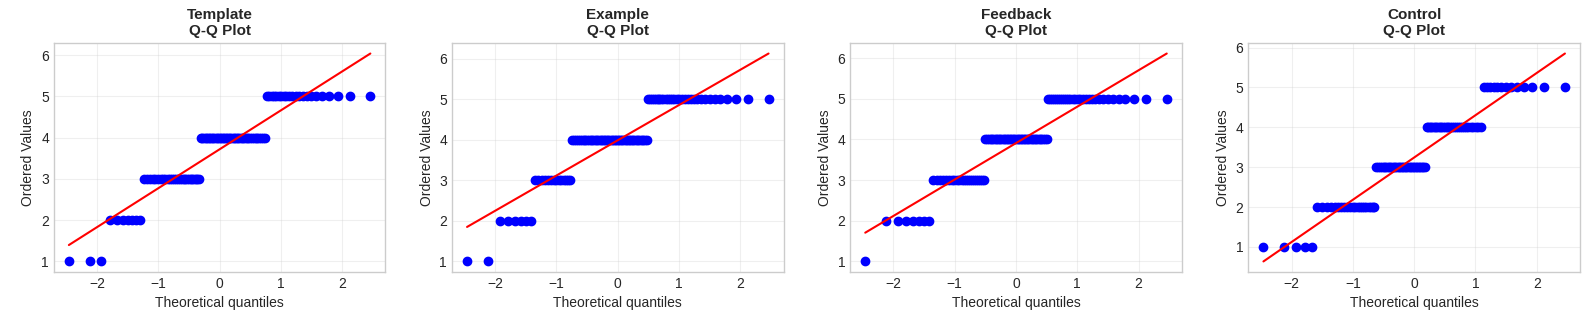
\includegraphics[width=0.9\textwidth]{figures/01.png}
\caption{Q-Q Plots of Effectiveness Scores Across Assistance Conditions}
\label{fig:qq_plots}
\end{figure}

Visual diagnostics reinforced the statistical findings. Q-Q (Quantile–Quantile) plots \autoref{fig:qq_plots} revealed systematic deviations from the reference line across all conditions, with notable clustering around middle ranges and departures at distributional extremes.  

\begin{figure}[h]
\centering
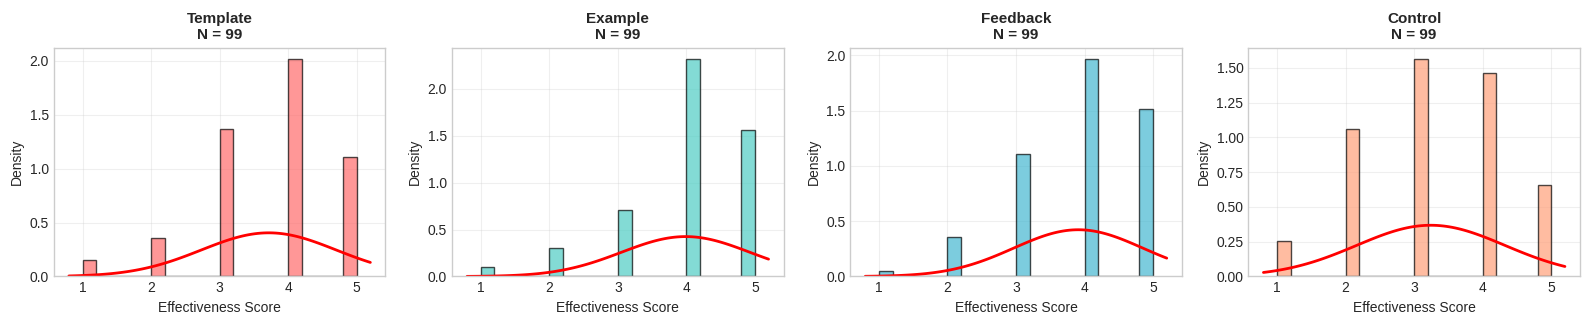
\includegraphics[width=0.9\textwidth]{figures/02.png}
\caption{Histograms of Effectiveness Scores Across Assistance Conditions}
\label{fig:histograms}
\end{figure}

Histograms with overlaid normal density curves \autoref{fig:histograms} demonstrated substantial divergence from theoretical normal distributions, exhibiting pronounced skewness and concentration at specific scale values. Example-based and feedback-based conditions showed heavy clustering at upper scores (4 and 5), while the control-based displayed greater dispersion around lower central values.

\begin{figure}[h]
\centering
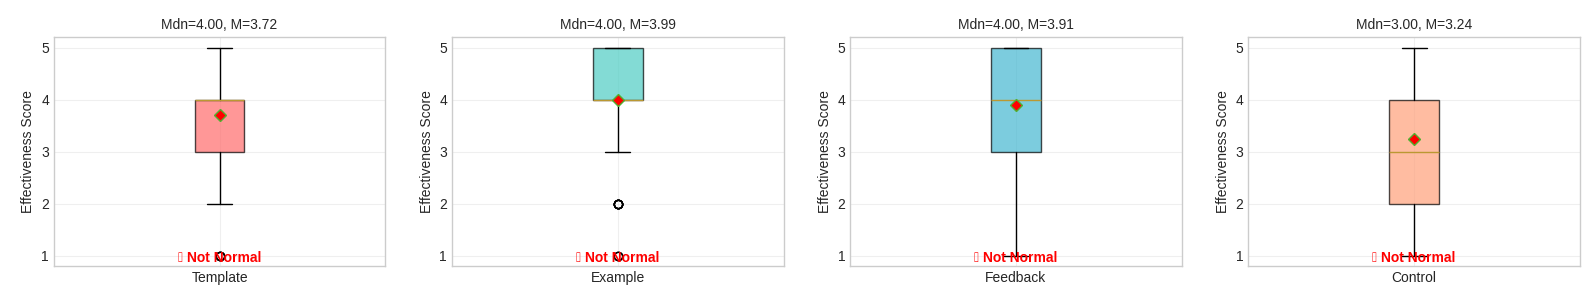
\includegraphics[width=0.9\textwidth]{figures/03.png}
\caption{Boxplots of Effectiveness Scores Across Assistance Conditions}
\label{fig:boxplots}
\end{figure}

Boxplots \autoref{fig:boxplots} further confirmed non-normality through irregular distributional shapes and outlier patterns inconsistent with Gaussian distributions. These convergent findings necessitated the adoption of non-parametric statistical approaches for all subsequent analyses, ensuring robust inference despite distributional violations.

\subsubsection{Descriptive Statistics:}

Central tendency and variability measures were calculated using medians and interquartile ranges (IQRs), preferred for ordinal Likert-scale data over means and standard deviations. \autoref{tab:descriptive_stats} presents comprehensive descriptive statistics for effectiveness ratings across all assistance conditions.

\begin{table}[h]
\centering
\begin{tabular}{lccccccc}
\hline
\textbf{Strategy} & \textbf{Median} & \textbf{Mean} & \textbf{SD} & \textbf{IQR} & \textbf{Min} & \textbf{Max} \\
\hline
Template & 3.67 & 3.72 & 0.78 & [3.33, 4.33] & 2.00 & 5.00 \\
Example & 4.00 & 3.99 & 0.74 & [3.67, 4.33] & 2.00 & 5.00 \\
Feedback & 4.00 & 3.91 & 0.64 & [3.67, 4.33] & 3.00 & 5.00 \\
Control & 3.33 & 3.24 & 0.72 & [3.00, 3.67] & 1.00 & 5.00 \\
\hline
\end{tabular}
\caption{Descriptive Statistics for Effectiveness Ratings by Assistance Condition}
\label{tab:descriptive_stats}
\end{table}

Example-based and feedback-based conditions achieved identical median effectiveness ratings (4.00), with narrow IQRs indicating consistent positive evaluations across participants. Both conditions demonstrated relatively low standard deviations (0.74 and 0.64, respectively), suggesting greater consensus regarding their utility.

Template-based assistance produced moderate effectiveness ratings (median = 3.67, M = 3.72), with a slightly wider distributional spread (IQR = [3.33, 4.33], SD = 0.78) compared to example-based and feedback-based assistance, indicating more variable participant responses.

The control condition yielded the lowest effectiveness evaluations (median = 3.33, M = 3.24), with the widest range (min = 1.00, max = 5.00) but moderate standard deviation (0.72), reflecting substantial between-participant variation in unassisted performance.

\subsection{\textbf{Primary Analysis}}

\subsubsection{Non-Parametric Analysis using the Friedman Test:}

The Friedman test is a non-parametric alternative to repeated measures ANOVA, designed to detect differences across multiple related groups when the assumption of normality is violated, as was the case in our study. It ranks the scores of each subject across conditions and evaluates whether these ranks differ systematically between groups. This repeated measures operates by ranking participant scores within conditions and tests whether rank distributions differ systematically across groups.

\begin{figure}[h]
\centering
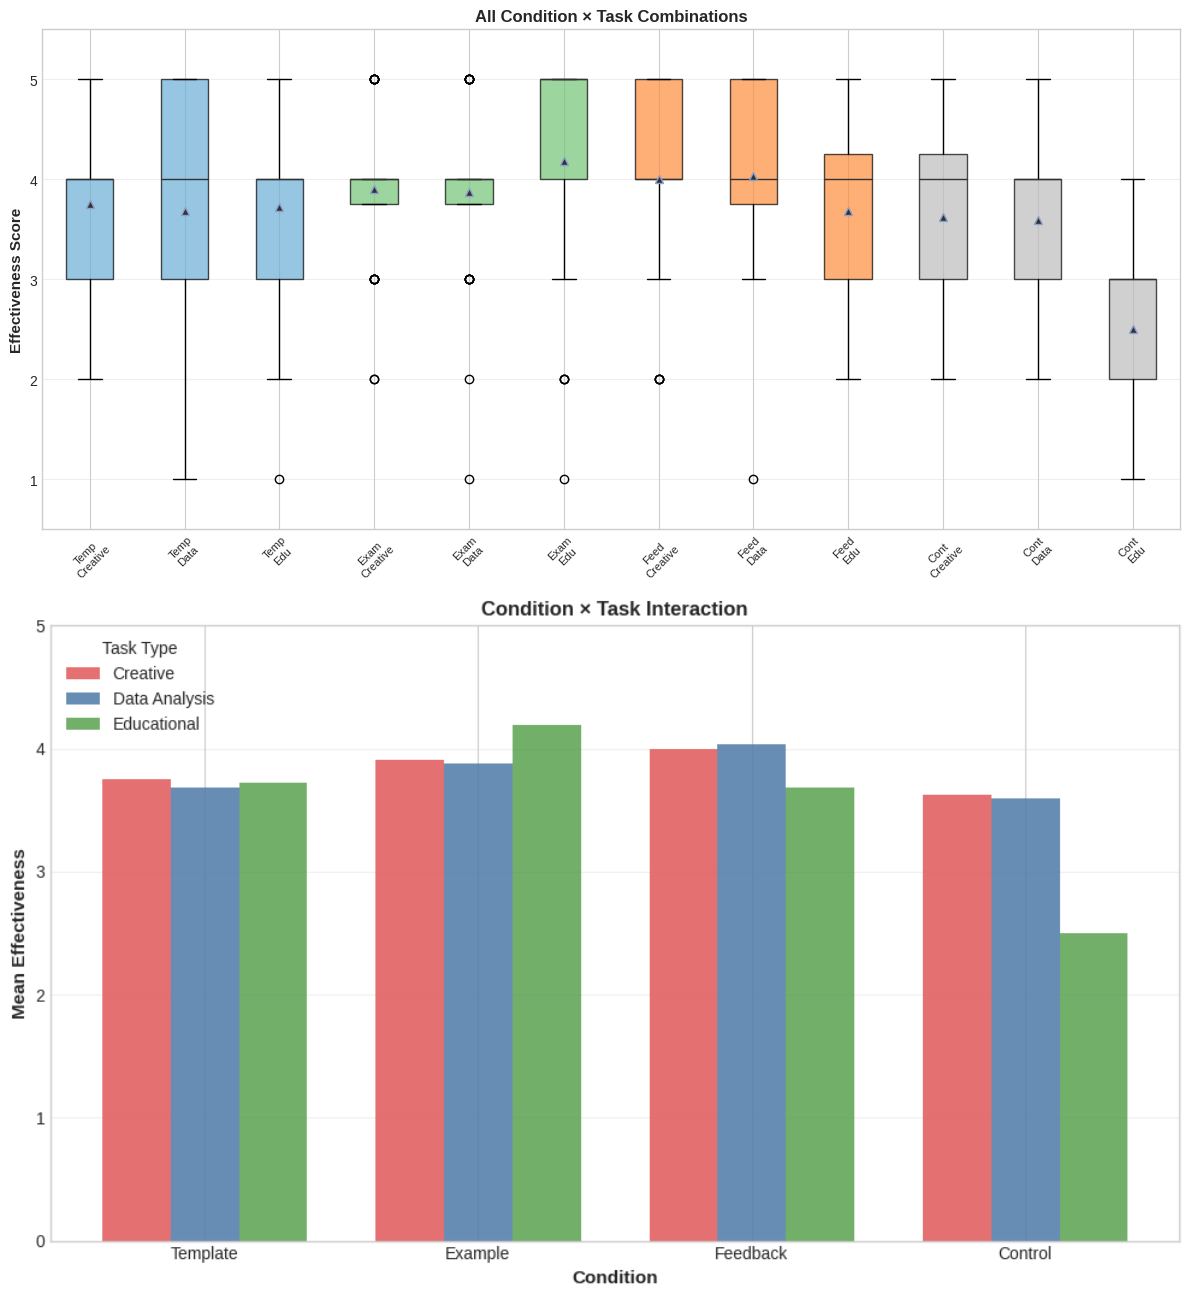
\includegraphics[width=0.6\textwidth]{figures/04.jpg}
\caption{Effectiveness of Assistance Conditions Across Task Domains: Boxplots and Bar Charts (Friedman Test Results)}
\label{fig:effectiveness_domains}
\end{figure}

\autoref{fig:effectiveness_domains} presents the effectiveness results across all condition × task combinations. The boxplots (top panel) illustrate the distribution of scores, while the bar chart (bottom panel) highlights condition × task interactions. Clear differences emerged between assistance conditions. Example-based and feedback-based support consistently produced higher median effectiveness scores, with concentrated ratings at the upper end of the scale, whereas template support yielded moderate improvements and control showed the lowest ratings with greater variability and several outliers. These differences confirm the Friedman test finding that assistance conditions significantly influenced perceived effectiveness.

Breaking the results down by task domain, example-based assistance was most effective in data analysis, where participants rated it highest for guiding them to structure prompts that extracted patterns and insights. Feedback-based assistance was most effective in educational tasks, reflecting its value in iteratively refining explanations for clarity and learner appropriateness. In creative writing, both example-based and feedback-based assistance outperformed template-based and control-based, though the differences were less pronounced compared to the other domains. Template-based support provided steady but modest benefits across all domains, helping participants cover essential details but not reaching the higher effectiveness levels of example-based or feedback-based assistance. By contrast, the control condition consistently underperformed, with the lowest ratings across all three domains, particularly in educational tasks where participants struggled most without guidance.

\subsubsection{Post-hoc Pairwise Comparisons:}

The Wilcoxon signed-rank test is a non-parametric post-hoc procedure that is widely applied after a Friedman test indicates significant differences across multiple conditions \cite{Benavoli2016Should} \cite{Xiang2022Large}. It evaluates whether the distribution of paired differences between two conditions is symmetric around zero by ranking the absolute differences, assigning signs, and testing whether the sum of signed ranks deviates significantly from what would be expected under the null hypothesis of no median difference.

\begin{figure}[h]
\centering
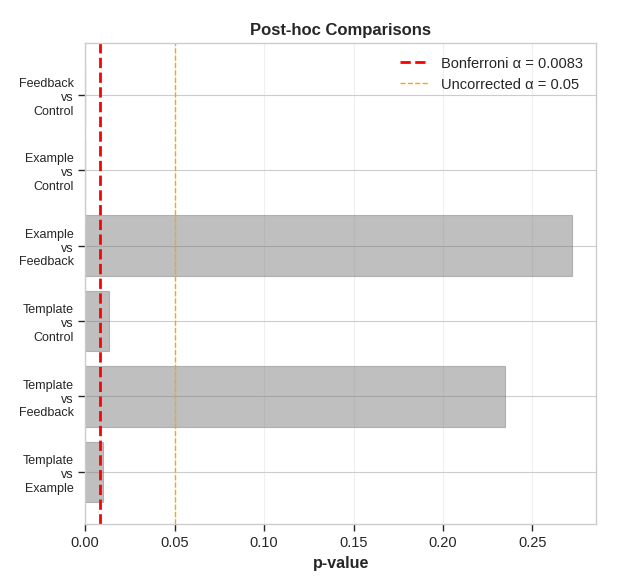
\includegraphics[width=0.7\textwidth]{figures/05.png}
\caption{Post-hoc Wilcoxon signed-rank Comparisons Across Assistance Conditions}
\label{fig:posthoc_wilcoxon}
\end{figure}

Following the significant Friedman test result, pairwise comparisons were conducted using the Wilcoxon signed-rank test, with the Bonferroni correction ($\alpha = 0.0083$) applied to adjust for multiple comparisons by dividing the overall significance level by the number of pairwise tests. The results, shown in \autoref{fig:posthoc_wilcoxon}, revealed that Template vs. Control and Feedback vs. Control both yielded highly significant differences ($p < 0.0083$), indicating that structured support in these conditions substantially improved effectiveness compared to no support. Example-based vs. control-based also showed a significant improvement, further confirming that unassisted prompting was consistently less effective. In contrast, Template vs. Example and Feedback vs. Example did not reach statistical significance, suggesting that although both Example and Feedback performed strongly, their difference was not large enough to be considered statistically reliable. Moreover, Example vs. Feedback produced the largest $p$-value ($> 0.25$), demonstrating clear similarity between these two conditions in terms of user-rated effectiveness. Overall, the post-hoc analysis reinforces the descriptive findings: example-based and feedback-based conditions substantially outperformed control and template-based, but did not differ significantly from each other, highlighting their comparable strength as structured assistance methods.

\subsubsection{Effect Size:}

Effect size measures provide an estimate of the magnitude of differences between conditions, complementing significance testing by indicating the practical importance of results \cite{in2024alternatives}. For Friedman tests, the recommended effect size is Kendall's W, which is calculated as:

\begin{equation}
W = \frac{\chi^2_{F}}{n (k-1)}
\end{equation}

where $\chi^2_{F}$ is the Friedman statistic, $n$ is the number of participants, and $k$ is the number of conditions. Kendall's W ranges from 0 (no agreement) to 1 (perfect agreement), with thresholds of 0.1, 0.3, and 0.5 typically interpreted as small, moderate, and large effects, respectively. In this study, Kendall's $W = 0.332$, indicating a moderate overall effect of the assistance strategy on effectiveness ratings. Reporting Kendall's W alongside significance testing provides interpretable evidence of practical significance \cite{in2024alternatives,tomczak2022need}.

\begin{figure}[h]
\centering
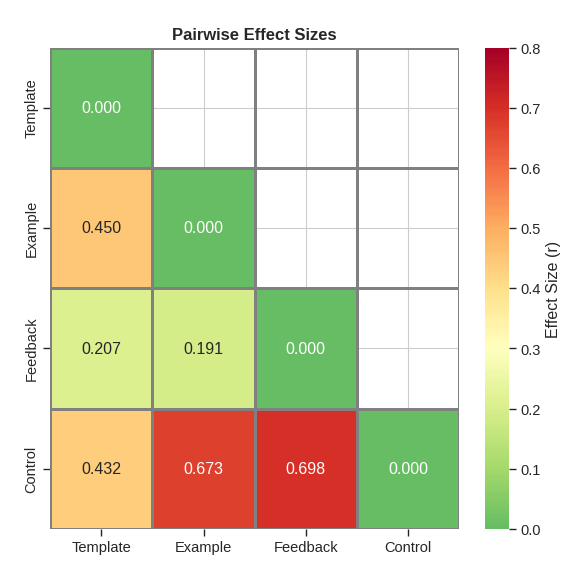
\includegraphics[width=0.6\textwidth]{figures/06.png}
\caption{Pairwise Effect Sizes (Wilcoxon signed-rank r) Across Assistance Conditions}
\label{fig:pairwise_effect_sizes}
\end{figure}

To complement this omnibus effect, pairwise effect sizes were also calculated for the Wilcoxon signed-rank comparisons using the correlation coefficient $r$. \autoref{fig:pairwise_effect_sizes} presents the pairwise effect size matrix, with values ranging from 0.0 (no effect) to $\sim$0.7 (large effect). The results highlight several important contrasts. Both Example vs. Control ($r = 0.673$) and Feedback vs. Control ($r = 0.698$) yielded large effect sizes, demonstrating substantial improvements in prompt effectiveness when structured assistance was provided compared to no support. Template vs. Control ($r = 0.432$) produced a moderate-to-large effect, indicating that even simple structured templates meaningfully improved outcomes relative to the baseline. By contrast, comparisons between the strongest assistance, such as Example vs. Feedback ($r = 0.191$), revealed only small effects, consistent with post-hoc tests showing no statistically significant difference between them. Example vs. Template ($r = 0.450$) and Feedback vs. Template ($r = 0.207$) showed small-to-moderate advantages, underscoring that while templates were beneficial, Example and Feedback assistance provided additional value.

Taken together, the effect size analysis reinforces the overall pattern: example-based and feedback-based assistance yielded the most substantial improvements, template-based offered moderate benefits, and the control-based condition consistently lagged behind. Importantly, these findings confirm that the impact of example and feedback assistance was not only statistically significant but also practically meaningful, with effect sizes indicating robust improvements in user effectiveness and experience.

\subsection{\textbf{Behavioral Measures}}
\subsubsection{Revision Frequency Across Assistance Conditions}
\FloatBarrier
\Needspace{:}

\begin{figure}[h]
\centering
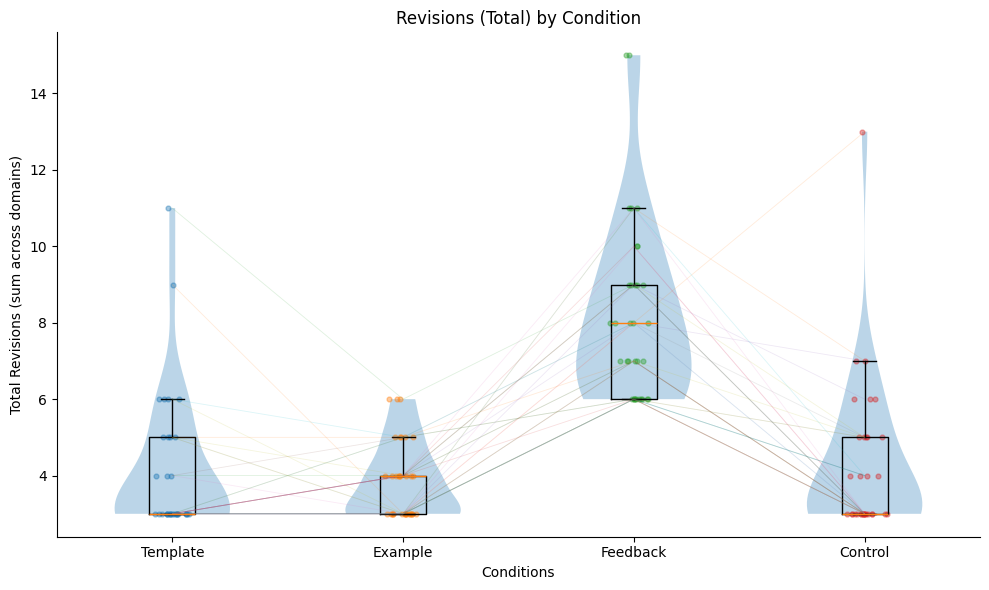
\includegraphics[width=0.7\textwidth]{figures/07.png}
\caption{Distribution of Total Revisions by Assistance Condition}
\label{fig:revision_frequency}
\end{figure}

The violin plot in \autoref{fig:revision_frequency} illustrates the total number of prompt revisions across the four assistance conditions. Revision frequency varied systematically by condition. The Feedback assistance produced the highest number of revisions, with a median of around 8 and several participants exceeding 12 revisions, indicating that iterative refinement was most actively pursued under this condition. The control condition also showed relatively high variability, with some participants making frequent revisions despite the absence of structured support. In contrast, the Template and Example assistance resulted in fewer revisions overall, with medians clustered between three and five edits, reflecting more concise revision behavior. These findings suggest that structured assistance, particularly feedback-based, encouraged participants to engage more extensively in iterative prompt refinement, whereas unguided and template-based conditions led to shorter and less variable revision processes.

\subsubsection{Time on Task Across Assistance Conditions}
\FloatBarrier
\usepackage{:}
\begin{figure}[h]
\centering
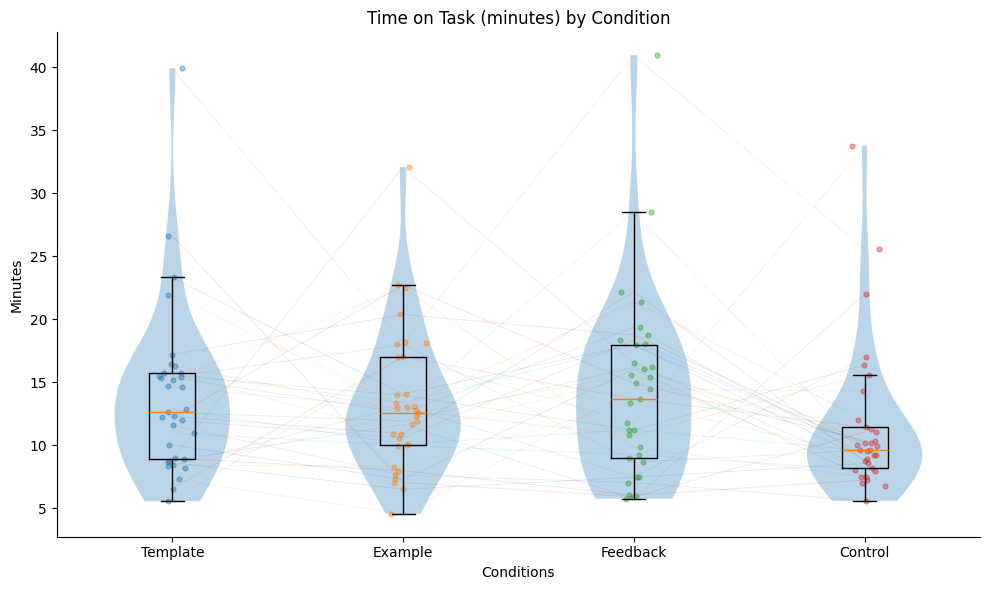
\includegraphics[width=0.7\textwidth]{figures/08.png}
\caption{Distribution of Time on Task (Minutes) by Assistance Condition}
\label{fig:time_on_task}
\end{figure}

In \autoref{fig:time_on_task} time on task varied across assistance conditions, with the Feedback condition showing the highest durations (median $\approx$ 15–18 minutes, with several participants exceeding 30 minutes), suggesting that iterative refinement required additional time. Template-based and example-based assistance showed moderate time investments (medians around 12–14 minutes), while the control condition resulted in the shortest completion times (median $\approx$ 9–10 minutes). These results indicate that structured support, particularly feedback-based guidance, led participants to spend more time engaging with tasks, whereas unguided conditions were completed more quickly but with less iterative depth.

\subsection{\textbf{Correlation Analysis}}

\subsubsection{Spearman's $\rho$ Correlation Analysis:}

We analyzed associations between participant factors (such as, digital literacy, confidence) and outcomes (such as, perceived effectiveness, satisfaction) using Spearman's rank correlation ($\rho$)—a non-parametric measure of monotonic association that does not assume normality and is well suited for ordinal survey data. Unlike Pearson's correlation, which requires interval data and normally distributed residuals, Spearman's $\rho$ operates on ranked data, making it robust against outliers and ties. This test is particularly recommended in survey-based human AI studies where Likert scales dominate and non-normality is common \cite{tyagi2022use,winter2024comparing}.

In the presence of ties, which are inevitable in Likert-scale data, Spearman's $\rho$ is defined as:

\begin{equation}
\rho = \frac{\text{cov}(R_X, R_Y)}{\sigma_{R_X} \, \sigma_{R_Y}}
\end{equation}

where $R_X$ and $R_Y$ are the ranked values of the two variables, $\text{cov}$ denotes covariance, and $\sigma$ indicates the standard deviation of the ranks \cite{upadhyay2021correlation}.

The computation was conducted using \texttt{scipy.stats.spearmanr}, which automatically ranks the data (assigning average ranks for ties), computes the covariance of ranks, and returns both the correlation coefficient and the $p$-value to test the null hypothesis $H_{0}: \rho = 0$. We applied this method to build a full correlation matrix, highlight statistically significant relationships, and visualize them with heatmaps and scatterplots as recommended by recent methodological work \cite{gu2022complex,briganti2024network}.

\begin{figure}[h]
\centering
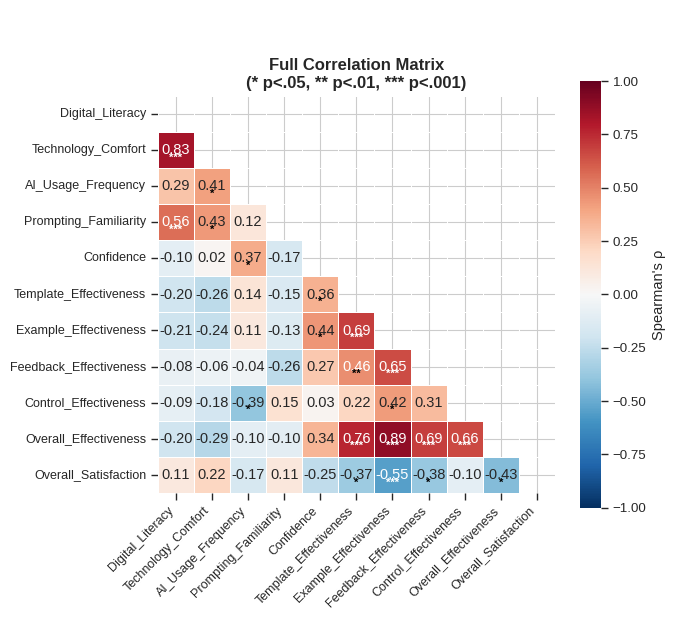
\includegraphics[width=0.65\textwidth]{figures/09.png}
\caption{Spearman Correlation Matrix of Predictor and Outcome Variables}
\label{fig:correlation_matrix}
\end{figure}

\autoref{fig:correlation_matrix} presents the full correlation matrix of participant characteristics and outcome measures. Several meaningful associations were observed. Technology comfort correlated strongly with prompting familiarity ($\rho = 0.83$, ***), indicating that participants more comfortable with technology were also more adept at constructing prompts. Confidence also showed positive associations with effectiveness ratings, particularly for Template ($\rho = 0.36$, *) and Example ($\rho = 0.44$, **), suggesting that self-assured participants benefited more from structured support. Effectiveness scores across conditions were positively interrelated, such as Example and Feedback ($\rho = 0.65$, ***), reflecting consistency in participants' evaluations. Overall effectiveness correlated positively with structured conditions ($\rho = 0.59–0.76$, ***), reinforcing the value of example-based and feedback-based support, while negative associations with individual challenge ratings suggested that stronger assistance reduced perceived difficulty. In contrast, digital literacy displayed only weak, non-significant correlations with outcomes, implying that task-specific confidence and comfort were more predictive of success than general digital skills. Collectively, these findings highlight that structured assistance, especially example-based and feedback-based assistance conditions, was reliably associated with higher effectiveness and satisfaction, moderated by participants' confidence and technology comfort.

\begin{figure}[h]
\centering
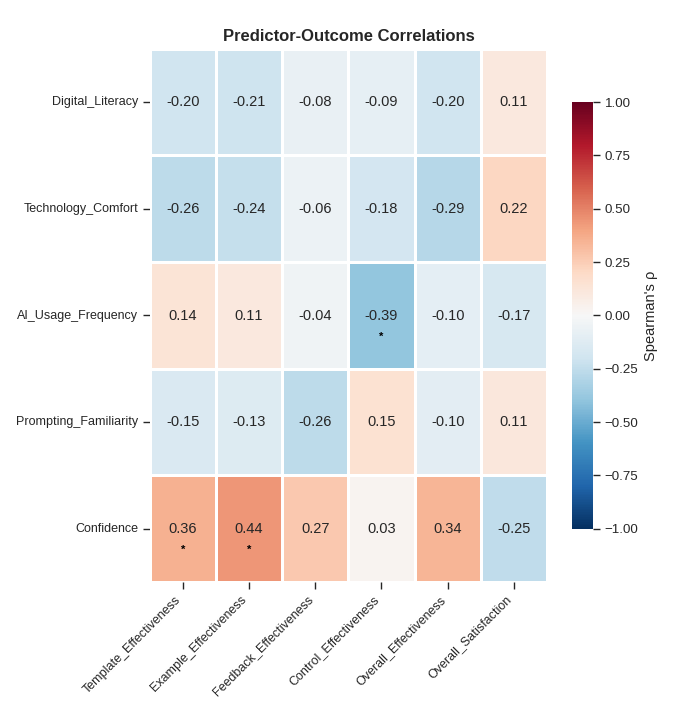
\includegraphics[width=0.4\textwidth]{figures/10.png}
\caption{Predictor Outcome Spearman Correlations}
\label{fig:predictor_outcome}
\end{figure}

\autoref{fig:predictor_outcome} illustrates the correlations between participant characteristics and outcome measures. Confidence emerged as the strongest positive predictor, showing significant associations with Example Effectiveness ($\rho = 0.44$, *), Template Effectiveness ($\rho = 0.36$, *), and Overall Effectiveness ($\rho = 0.34$). This indicates that participants who were more confident tended to produce more effective prompts when supported by structured assistance conditions. In contrast, AI usage frequency correlated negatively with Control Effectiveness ($\rho = –0.39$, *), suggesting that participants with greater prior experience using AI tools rated unguided prompting less favorably. Other predictors, such as technology\_comfort and prompting\_familiarity, displayed only weak, non-significant associations, while digital\_literacy showed negligible relationships with outcomes. Collectively, these findings emphasize that task-specific confidence, rather than general digital skills or technology familiarity, played the most critical role in shaping perceptions of effectiveness and satisfaction with the assistance conditions.


\begin{figure}[h]
\centering
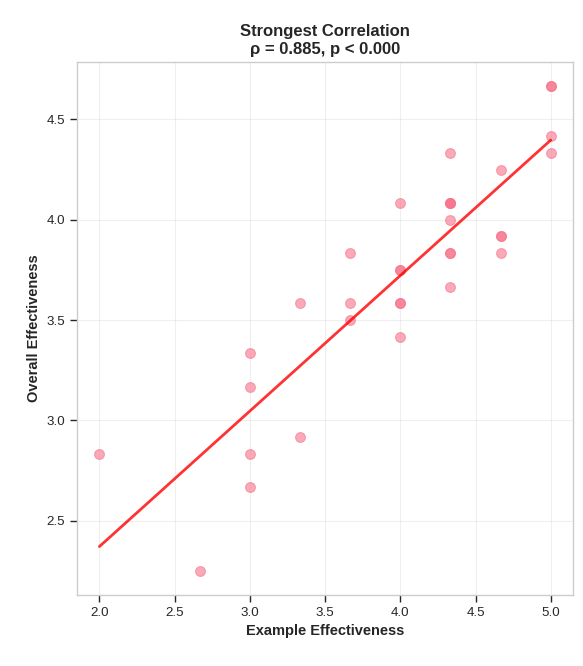
\includegraphics[width=0.3\textwidth]{figures/11.png}
\caption{Strongest Correlation Between Example Effectiveness and Overall Effectiveness}
\label{fig:strongest_correlation}
\end{figure}

\autoref{fig:strongest_correlation} depicts the strongest association observed in the dataset, between Example Effectiveness (x-axis) and Overall Effectiveness (y-axis). The correlation was exceptionally strong ($\rho = 0.885$, $p < .001$), demonstrating a highly significant positive monotonic relationship. The fitted regression line illustrates a clear upward trend, indicating that participants who perceived example-based assistance as more effective also tended to evaluate their overall task performance more positively. This finding underscores that example-based support was not only rated as highly effective within individual tasks but also emerged as the strongest predictor of overall success, highlighting its central role among the assistance conditions.

\begin{figure}[h]
\centering
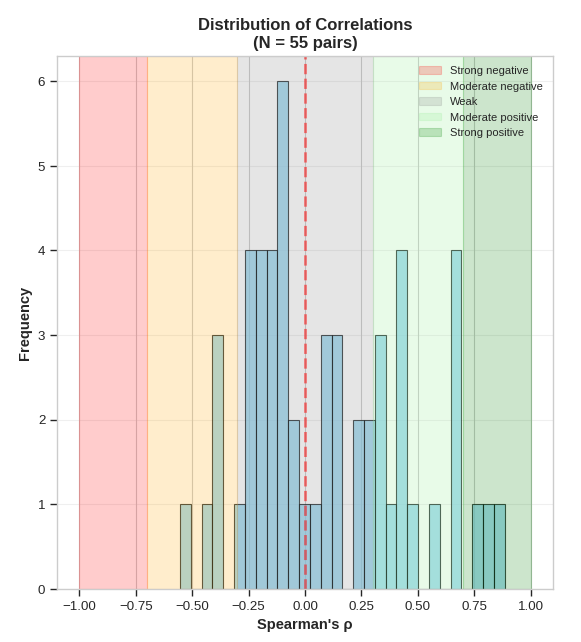
\includegraphics[width=0.4\textwidth]{figures/12.png}
\caption{Distribution of Spearman's Correlation Coefficients Across Variable Pairs}
\label{fig:correlation_distribution}
\end{figure}

\autoref{fig:correlation_distribution} displays the distribution of all 55 Spearman's $\rho$ values calculated across variable pairs in the dataset. The x-axis ranges from –1 (perfect negative association) to +1 (perfect positive association), while the y-axis indicates the frequency of correlations within each bin. Colored bands mark interpretive thresholds, from strong negative ($\rho \leq –0.7$) to strong positive ($\rho \geq 0.7$), with the dashed vertical line denoting zero correlation. Most correlations clustered in the weak to moderate range, suggesting modest associations between participant characteristics and outcomes. A smaller subset of strong positive correlations was observed, particularly those involving example effectiveness, while strong negative associations were rare. This distribution provides an overall perspective on the relational structure of the dataset, complementing the more detailed patterns illustrated by the correlation heatmaps and scatterplots.

% Bibliography references used in the text
\bibliographystyle{plain}
% Note: You would need to add these references to your .bib file
% [22] Benavoli et al. 2016
% [18] In et al. 2024  
% [19] Tomczak & Tomczak 2022
% [29] Tyagi et al. 2022
% [30] Winter et al. 2024
% [31] Upadhyay & Shukla 2021
% [32] Gu 2022
% [33] Briganti et al. 2024
\section{\textbf{Discussion}}

Overall, the analyses showed that feedback-based assistance prompted the most revisions and longest task durations, reflecting deeper iterative engagement, while example-based assistance achieved the highest effectiveness ratings and was the strongest predictor of overall success. Template-based support offered moderate benefits, improving outcomes relative to control but remaining less effective than the other two strategies. Control consistently lagged behind, with faster but less effective task performance.

\subsection {\textbf {Response to the Research Question}}
Structured assistance consistently outperformed no assistance across domains, with example-based and feedback-based strategies providing the strongest benefits. Example-based support was most effective for data analysis, while feedback-based support was most effective for educational content; in creative writing, both strategies outperformed templates and control, though differences were smaller. These findings indicate that assistance should be matched to task type, such as, examples are particularly beneficial for analytical tasks, feedback best supports instructional or explanatory tasks, and both reliably surpass templates and control.

\subsection {\textbf {Implications}}
The findings suggest that LLM-assisted interfaces should adopt domain aware defaults, offering example galleries for data analysis and iterative feedback tools for educational tasks. Since example and feedback based strategies are equally strong, systems should let users combine or switch between them, such as starting with examples and refining with feedback. Given the time quality trade-off of feedback, interfaces can frame it as a “deeper refinement mode” with time cues to manage effort. Support should also be confidence-adaptive: lighter templates for confident users, stronger helps for less confident ones. Finally, systems should evaluate both subjective effectiveness and behavioral signals to capture impact comprehensively and inform design.

\subsection {\textbf {Limitations}}
The within-subjects design enabled direct comparisons but introduced potential fatigue effects across the 12 conditions, which may have reduced participant engagement in later trials. The quality of LLM outputs was assessed through participants’ self-reported ratings, which reflect subjective perceptions rather than an objective scientific evaluation. Finally, the relatively small sample of 33 participants, drawn from a single educational and technical context, limits the generalizability of the findings to more diverse populations.

\subsection {\textbf {Future Work}}
Future research should address these limitations through several methodological enhancements. Implementing a mixed-methods approach combining quantitative effectiveness ratings with qualitative analysis of prompt revisions would illuminate the mechanisms through which different assistance conditions influence user behavior. Incorporating automated quality assessment of outputs would validate whether perceived effectiveness translates to measurable improvement. Larger and more diverse samples would enhance external validity as well. Future investigations should explore adaptive assistance systems that adjust support based on user confidence and task complexity. The optimal combinations of assistance conditions, such as beginning with example-based assistance and then transitioning to feedback-based refinement, might yield superior results to single-strategy approaches.

\subsection {\textbf {Conclusion}}
This study offers the systematic comparison of multiple assistance conditions for prompt revision across diverse LLM task domains, showing that structured support meaningfully improves outcomes over unguided revision. Beyond demonstrating the relative advantages of example and feedback-based approaches, the findings establish that even minimal scaffolds, such as templates, provide value for certain users and contexts. These results extend the growing literature on human–LLM interaction by highlighting the importance of aligning assistance design with task characteristics. Overall, the study underscores that effective prompt revision is not simply a matter of user persistence, but of providing the right kind of structured support to unlock the full potential of LLMs.


\bibliographystyle{ACM-Reference-Format}
\bibliography{sample-base}

\end{document}